\documentclass{article}
\usepackage{fancyhdr}
\usepackage{ctex}
\usepackage{listings}
\usepackage{graphicx}
\usepackage[a4paper, body={18cm,22cm}]{geometry}
\usepackage{amsmath,amssymb,amstext,wasysym,enumerate,graphicx}
\usepackage{float,abstract,booktabs,indentfirst,amsmath}
\usepackage{array}
\usepackage{booktabs}
\usepackage{multirow}
\usepackage{url}
\usepackage{diagbox}
\renewcommand\arraystretch{1.4}
\usepackage{indentfirst}
\setlength{\parindent}{2em}
\usepackage{enumitem}
\setmonofont{DejaVu Sans Mono}
\usepackage{listings}
\usepackage{xcolor}
\usepackage{makecell}
\setCJKmonofont{黑体}
\usepackage{tikz}
\usepackage{tabularx}
\usepackage{amsmath}
\usetikzlibrary{positioning, arrows.meta}
\lstset{
    % language = C,
    xleftmargin = 3em,xrightmargin = 3em, aboveskip = 1em,
	backgroundcolor = \color{white}, % 背景色
	basicstyle = \small\ttfamily, % 基本样式 + 小号字体
	rulesepcolor= \color{gray}, % 代码块边框颜色
	breaklines = true, % 代码过长则换行
	numbers = left, % 行号在左侧显示
	numberstyle = \small, % 行号字体
    numbersep = -14pt, 
    keywordstyle=\color{purple}\bfseries, % 关键字颜色
    commentstyle =\color{red!50!green!50!blue!60}, % 注释颜色
    stringstyle = \color{red}, % 字符串颜色
    morekeywords={ASSERT, int64_t, uint32_t},
	frame = shadowbox, % 用(带影子效果)方框框住代码块
	showspaces = false, % 不显示空格
	columns = fixed, % 字间距固定
} 
\lstset{
    sensitive=true,
    moreemph={ASSERT, NULL}, emphstyle=\color{red}\bfseries,
    moreemph=[2]{int64_t, uint32_t, tid_t, uint8_t, int16_t, uint16_t, int32_t, size_t}, emphstyle=[2]\color{purple}\bfseries,
    }
%--------------------页眉--------------------%
\pagestyle{fancy}
\fancyhead[L]{}
\fancyhead[R]{}
\fancyhead[C]{华东师范大学软件工程学院实验报告}
\fancyfoot[C]{-\thepage-}
\renewcommand{\headrulewidth}{1.5pt}
%--------------------标题--------------------%
\begin{document}
\begin{center}
    \LARGE{{\textbf{\heiti 华东师范大学软件工程学院实验报告}}}
    \begin{table}[H]
        \centering
        \begin{tabular}{p{2cm}p{4cm}<{\centering}p{1cm}p{2cm}p{4cm}<{\centering}}
            实验课程:    & 计算机网络 & \quad & 年\qquad 级: & 2022级               \\ \cline{2-2} \cline{5-5}
            实验编号:    & Lab 07     & \quad & 实验名称:    & \texttt{socket} 编程
            \\ \cline{2-2} \cline{5-5}
            姓\qquad 名: & 李鹏达     & \quad & 学\qquad 号: & 10225101460          \\ \cline{2-2} \cline{5-5}
        \end{tabular}
    \end{table}
\end{center}
\rule{\textwidth}{1pt}
%--------------------正文--------------------%
\section{实验目的}
\begin{enumerate}[noitemsep, label={{\arabic*})}]
    \item 熟悉 \texttt{socket} 编程的基本原理
    \item 掌握简单的套接字编程
    \item 掌握通过 \texttt{socket} 编程实现 \texttt{C/S} 程序的基本方法
    \item 了解应用层和运输层的作用及相关协议的工作原理和机制

\end{enumerate}
\section{实验内容与实验步骤}
\subsection{实验内容}

实现 \texttt{Client} 和 \texttt{Server} 的通信,并满足以下要求:

\begin{table}[H]
    \centering
    \begin{tabularx}{0.95\textwidth}{|X|X|X|X|X|X|X|X|X|X|}
        \hline
        \multicolumn{3}{|X|}{\texttt{Server}} & \multicolumn{3}{|X|}{\texttt{Client}}   & \multicolumn{3}{|X|}{整个系统}   & \texttt{Bonus}                                                                                                                                                                                                                                                    \\
        \hline
        能在标准输出打印客户端发送的消息      & 支持5个以上客户端同时发送消息并逐一打印 & 绑定至错误的端口号时提示出错信息 & 能从标准输入或文件接收信息 & 标准输入信息以两次回车作为结束标志 & 连接至错误的 \texttt{IP} 地址/端口号时能提示错误信息 & 支持在 \texttt{local host} 及两台不同机器上运行 & 支持长文本消息(不少于 \texttt{20KB}),有缓冲区管理 & 容错性好,无闪退 & 支持双工通信 \\
        \hline
    \end{tabularx}
\end{table}

\subsection{实验步骤}

\subsubsection{创建 \texttt{socket}}

在 \texttt{Linux} 下,使用 \texttt{sys/socket.h} 头文件(\texttt{Windows} 下是 \texttt{winsock2.h}) 中的 \texttt{socket} 函数创建一个套接字。(在 \texttt{Windows} 下需要先调用 \texttt{WSAStartup} 进行准备)

\begin{lstlisting}[language=C++, title=创建套接字]
        socket() : m_descriptor(-1) {
    #ifdef _WIN32
            WSADATA wsa_data;
            if (WSAStartup(MAKEWORD(2, 2), &wsa_data) != 0) {
                throw std::runtime_error("WSAStartup failed");
            }
    #endif
            m_descriptor = ::socket(AF_INET, SOCK_STREAM, 0);
            if (m_descriptor < 0) {
                throw std::runtime_error("create socket failed");
            }
        } 
\end{lstlisting}

其中,\texttt{AF\_INET} 表示使用 \texttt{IPv4} 协议,\texttt{SOCK\_STREAM} 表示使用 \texttt{TCP} 协议。

\subsubsection{\texttt{bind}}

使用 \texttt{bind} 函数将套接字与端口号绑定。

\begin{lstlisting}[language=C++, title=bind]
    void bind(int port) {
        if (port < 0 || port > 65535) {
            m_close_socket();
            throw std::runtime_error("invalid port");
        }

        sockaddr_in server_addr;
        server_addr.sin_family = AF_INET;
        server_addr.sin_addr.s_addr = INADDR_ANY;
        server_addr.sin_port = htons(port);

        if (::bind(m_descriptor, (sockaddr *)&server_addr,
                  sizeof(server_addr)) == -1) {
            m_close_socket();
            throw std::runtime_error(
                "bind to port " + std::to_string(port) +
                " failed\n maybe the port is already in use");
        } else {
            m_info("bind to port " + std::to_string(port));
        }
    }
\end{lstlisting}

\subsubsection{\texttt{listen}}

使用 \texttt{listen} 函数监听端口。

\begin{lstlisting}[language=C++, title=listen]
    void listen(int n = 10) {
        if (::listen(m_descriptor, n) == -1) {
            m_close_socket();
            throw std::runtime_error("listen socket failed");
        } else {
            m_info("listening");
        }
    }
\end{lstlisting}

其中,\texttt{n}表示最大连接数。

\subsubsection{\texttt{accept}}

使用 \texttt{accept} 函数接受客户端的连接。

\begin{lstlisting}[language=C++, title=accept]
    int accept() {
        sockaddr_in client_addr;
        socklen_t client_addr_len = sizeof(client_addr);
        int connected =
            ::accept(m_descriptor, (sockaddr *)&client_addr, &client_addr_len);
        if (connected == -1) {
            m_close_socket();
            throw std::runtime_error("accept socket failed");
        } else {
            m_info("accept socket id " + std::to_string(connected) + " from " +
                  std::string(inet_ntoa(client_addr.sin_addr)) + ":" +
                  std::to_string(ntohs(client_addr.sin_port)));
        }
        return connected;
    }
\end{lstlisting}

\subsubsection{\texttt{connect}}

使用 \texttt{connect} 函数主动与服务器建立连接。

\begin{lstlisting}[language=C++, title=connect]
    int connect(const char *ip, int port) {
        sockaddr_in server_addr;
        server_addr.sin_family = AF_INET;
        server_addr.sin_addr.s_addr = inet_addr(ip);
        server_addr.sin_port = htons(port);

        int connected = ::socket(AF_INET, SOCK_STREAM, 0);

        if (::connect(connected, (sockaddr *)&server_addr,
                      sizeof(server_addr)) == -1) {
            m_close_socket();
            throw std::runtime_error("connect to " + std::string(ip) + ":" +
                                    std::to_string(port) + " failed");
        } else {
            m_info("connect to " + std::string(ip) + ":" +
                  std::to_string(port));
        }
        return connected;
    }

    int connect(std::string_view ip, int port) {
        return connect(ip.data(), port);
    }
\end{lstlisting}

\subsubsection{\texttt{send}}

使用 \texttt{send} 函数发送数据。

\begin{lstlisting}[language=C++, title=send]
    void send(int to, const char *data, int len) {
        if (::send(to, data, len, 0) == -1) {
            m_error("send data to " + std::to_string(to) + " failed");
        }
    }

    void send(int to, std::string_view data) {
        send(to, data.data(), data.size());
    }
\end{lstlisting}

\subsubsection{\texttt{recv}}

使用 \texttt{recv} 函数接收数据。

\begin{lstlisting}[language=C++, title=recv]
    bool recv(int from, char *data, int len) {
        int read_num = ::recv(from, data, len, 0);
        if (read_num == -1) {
            m_error("recv data from " + std::to_string(from) + " failed");
            return false;
        }
        if (read_num == 0) {
            return false;
        }
        return true;
    }
\end{lstlisting}

\subsubsection{\texttt{close}}

使用 \texttt{close} 函数关闭套接字。

\begin{lstlisting}[language=C++, title=close]
    void m_close_socket() {
        if (m_descriptor != -1) {
            m_info("socket closed");
            ::close(m_descriptor);
            m_descriptor = -1;
        }
    }

    // ...

    ~socket() {
        m_close_socket();
    }

    void close() {
        m_close_socket();
    }
\end{lstlisting}

\section{实验环境}
\texttt{Windows} 下:
\begin{itemize}[noitemsep]
    \item \texttt{Windows 11 家庭中文版 23H2 22631.2715}
    \item \texttt{gcc version 13.2.0 (MinGW-W64 x86\_64-ucrt-mcf-seh, built by Brecht Sanders)}
    \item \texttt{GNU Make 3.81}
\end{itemize}

\texttt{Linux} 下:

\begin{itemize}[noitemsep]
    \item \texttt{Ubuntu 22.04.3 LTS on Windows 10 x86\_64}
    \item \texttt{gcc version 11.4.0 (Ubuntu 11.4.0-1ubuntu1~22.04)}
    \item \texttt{GNU Make 4.3}
\end{itemize}


\section{实验结果与分析}

\subsection{\texttt{Server}}

\subsubsection{能在标准输出打印客户端发送的消息}

在收到消息后打印即可。

\begin{lstlisting}[language=C++]
    void handle_connection(socket_server &socket, int client) {
        while (true) {
            auto msg = socket.recv(client);
            if (msg.empty()) {
                break;
            }
            std::cout << "server received from " << client << ": " << msg
                      << std::endl;
            msg = msg.substr(0, msg.size() - 1);
            socket.send_all(msg == "\n" ? "" : msg);
            socket.send_all("");
        }
    }
\end{lstlisting}

\begin{figure}[H]
    \centering
    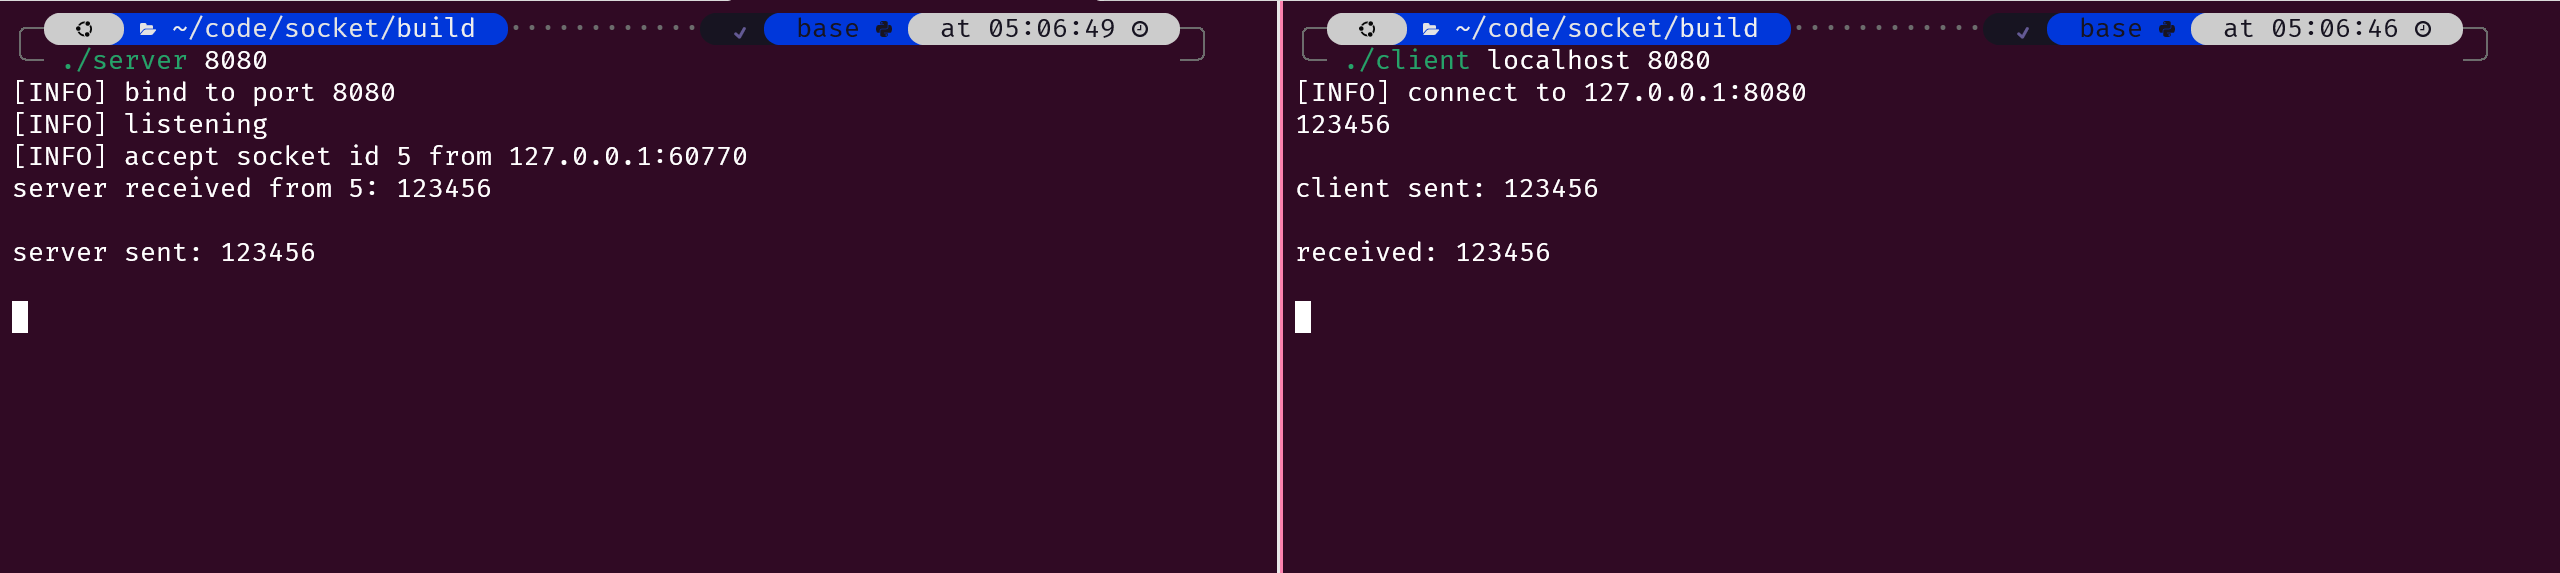
\includegraphics[width=0.95\textwidth]{img/1.png}
    \caption{能在标准输出打印客户端发送的消息}
\end{figure}

\subsubsection{支持5个以上客户端同时发送消息并逐一打印}

使用多线程,每个线程处理一个客户端的连接。

\begin{lstlisting}[language=C++]
    socket_server server{};

    server.bind(port);
    server.listen();

    std::vector<std::thread> threads{};

    while (true) {
        int client = server.accept();
        threads.emplace_back(handle_connection, std::ref(server), client);
    }

    for (auto &thread : threads) {
        thread.join();
    }
\end{lstlisting}

\begin{figure}[H]
    \centering
    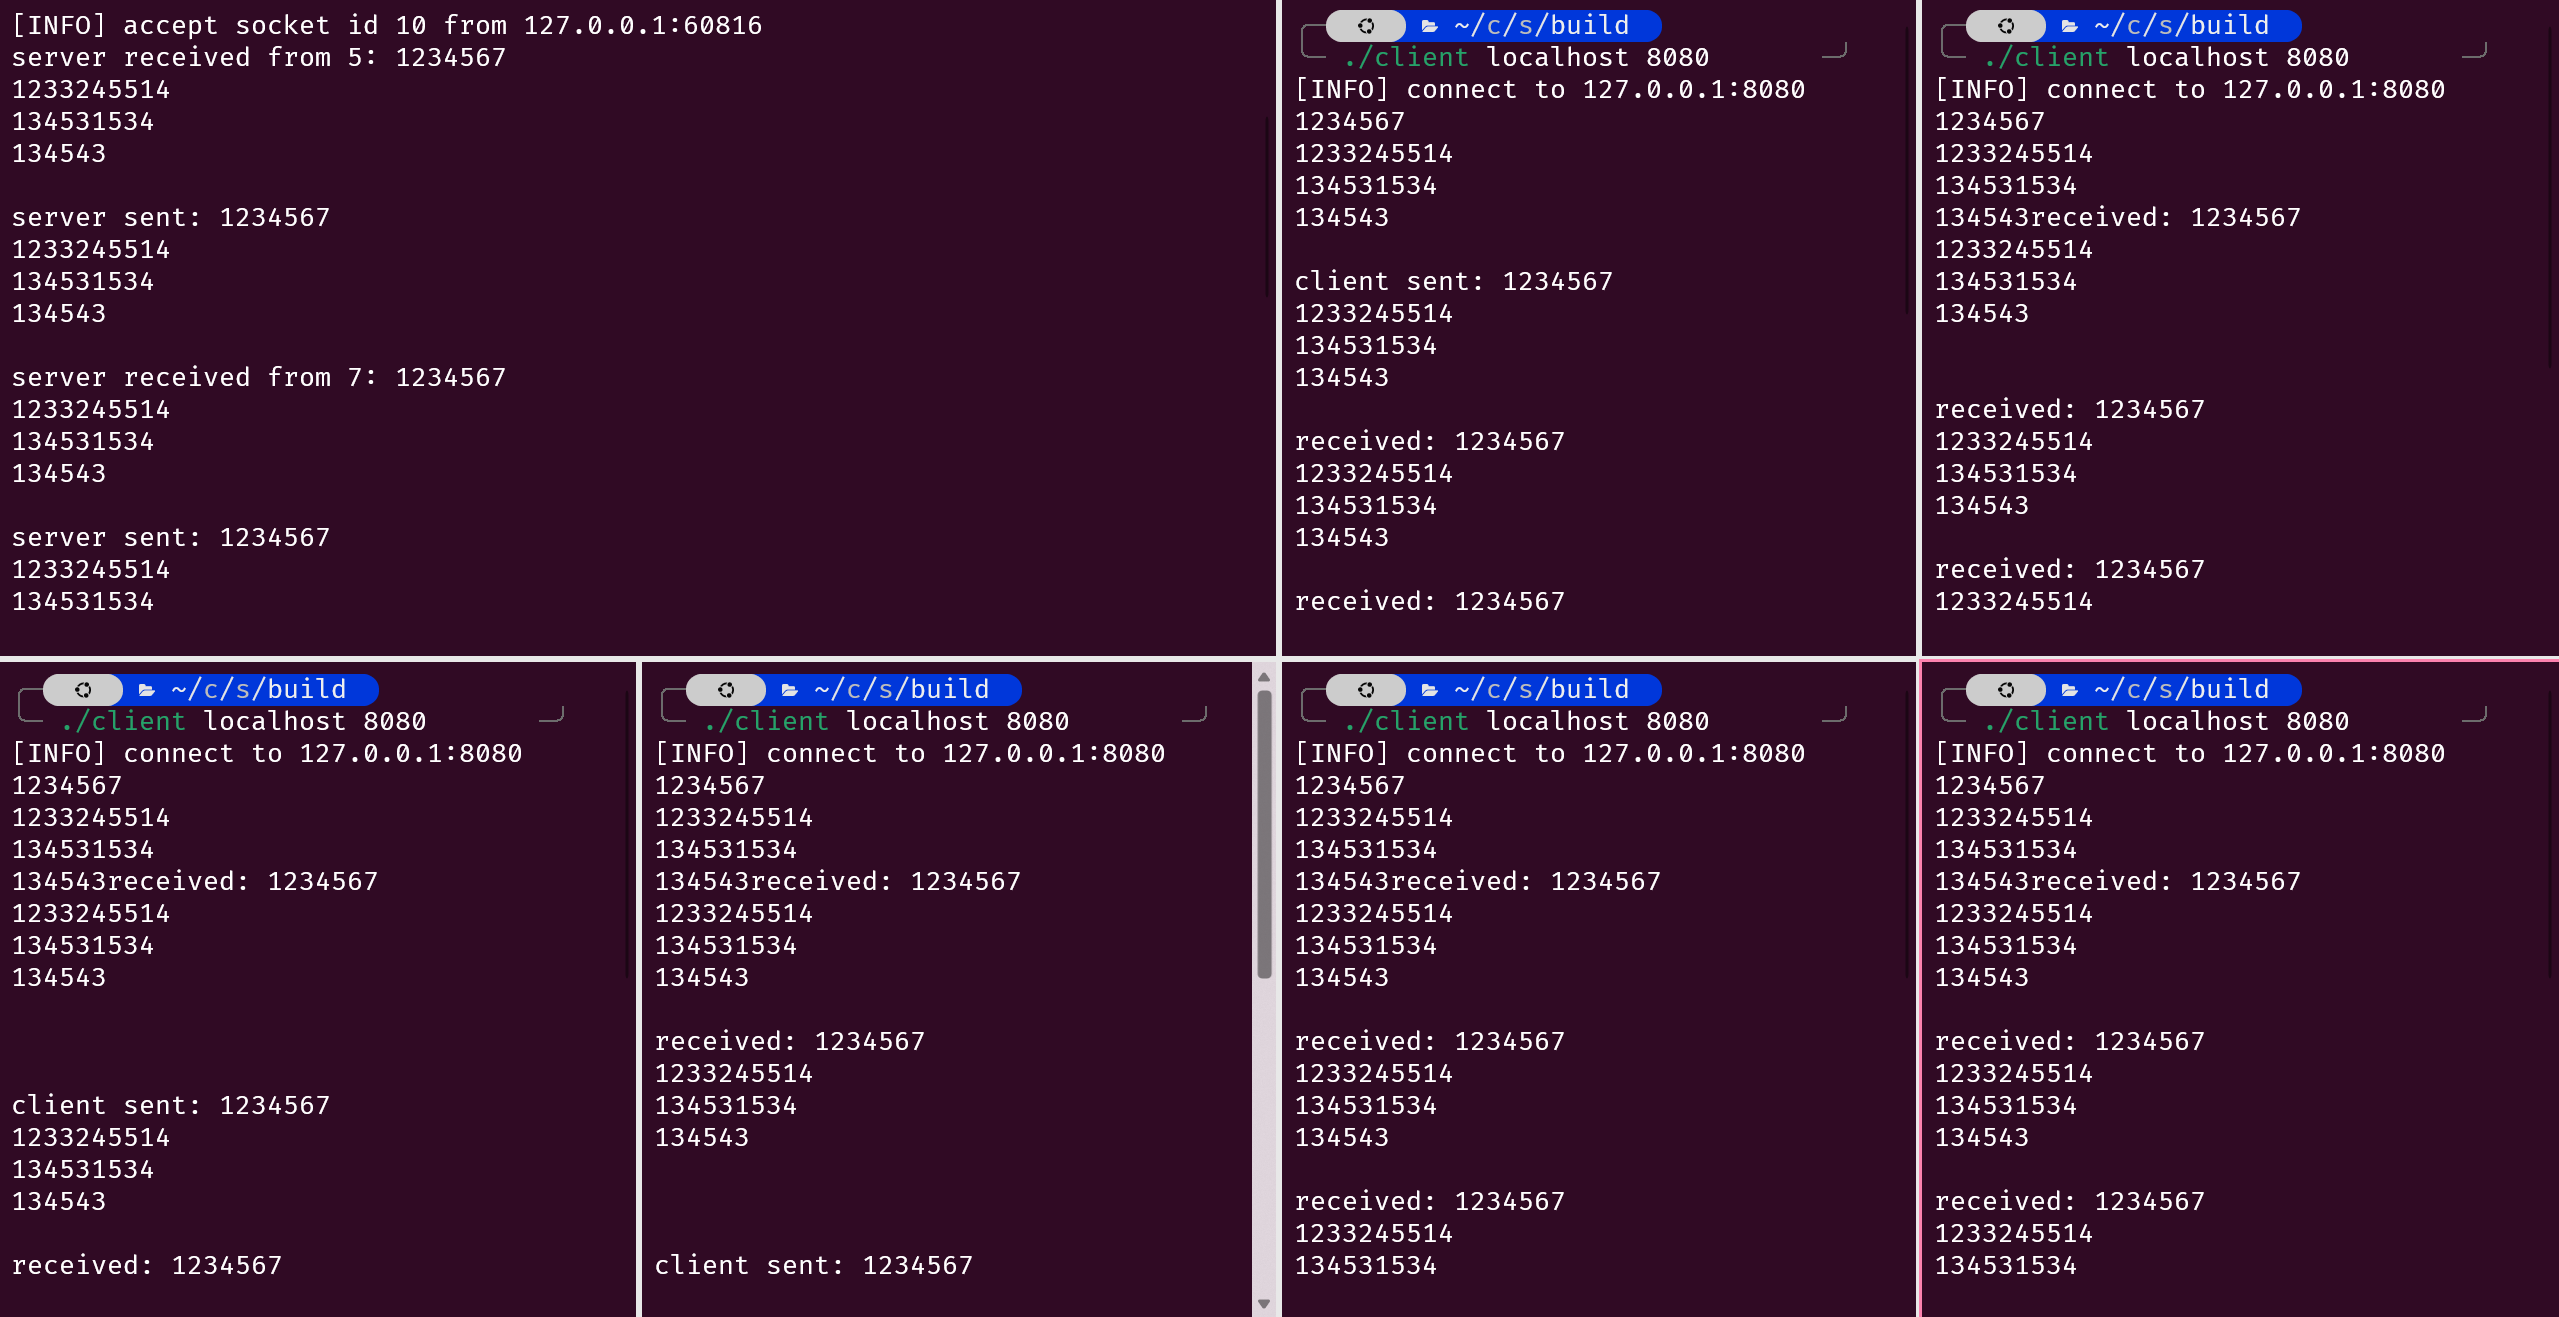
\includegraphics[width=0.95\textwidth]{img/2.png}
    \caption{支持5个以上客户端同时发送消息并逐一打印}
\end{figure}

\subsubsection{绑定至错误的端口号时提示出错信息}

对端口号进行检查,并在 \texttt{bind} 失败时抛出异常。

\begin{lstlisting}[language=C++]
    void bind(int port) {
        if (port < 0 || port > 65535) {
            m_close_socket();
            throw std::runtime_error("invalid port");
        }

        sockaddr_in server_addr;
        server_addr.sin_family = AF_INET;
        server_addr.sin_addr.s_addr = INADDR_ANY;
        server_addr.sin_port = htons(port);

        if (::bind(m_descriptor, (sockaddr *)&server_addr,
                  sizeof(server_addr)) == -1) {
            m_close_socket();
            throw std::runtime_error(
                "bind to port " + std::to_string(port) +
                " failed\n maybe the port is already in use");
        } else {
            m_info("bind to port " + std::to_string(port));
        }
    }

    // ...

    int port{-1};
    try {
        port = std::stoi(argv[1]);
    } catch (std::exception &e) {
        std::cerr << "Invalid port" << std::endl;
        show_usage();
        return 1;
    }

    if (port < 0 || port > 65535) {
        std::cerr << "Invalid port" << std::endl;
        show_usage();
        return 1;
    }
\end{lstlisting}

\begin{figure}[H]
    \centering
    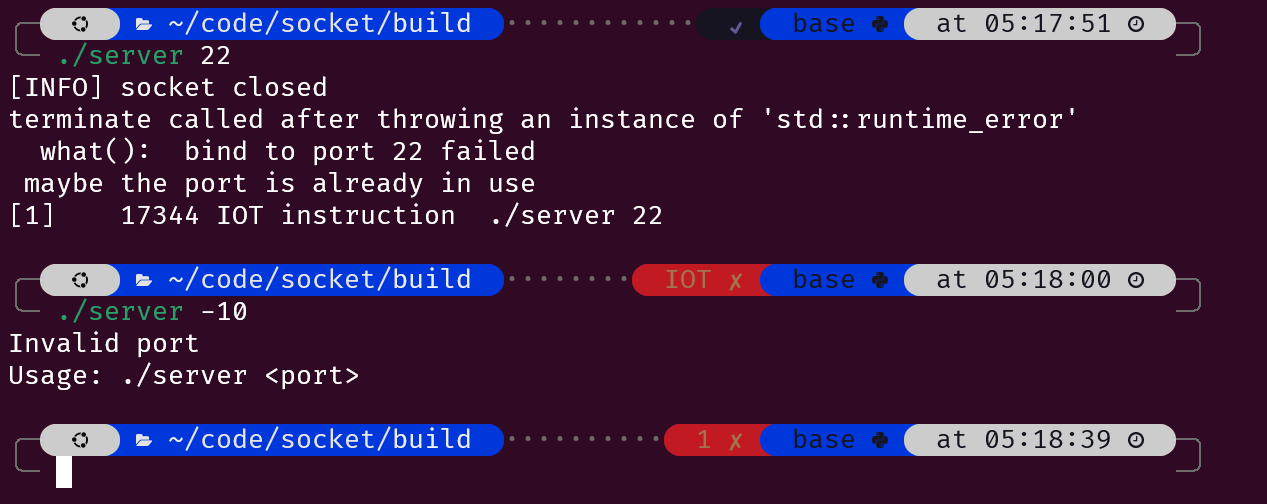
\includegraphics[width=0.95\textwidth]{img/3.png}
    \caption{绑定至错误的端口号时提示出错信息}
\end{figure}

\subsection{\texttt{Client}}

\subsubsection{能从标准输入或文件接收信息}

使用 \texttt{getline} 函数从标准输入读取信息。

\begin{lstlisting}[language=C++]
    while (true) {
        std::string msg;
        std::getline(std::cin, msg);
        client.send(msg);
    }
\end{lstlisting}

使用 \texttt{std::fstream} 从文件流读取信息。

\begin{lstlisting}[language=C++]
    if (argc == 5) {
        std::fstream in{argv[4]};
        std::string str{};
        std::string tmp{};
        while (std::getline(in, tmp)) {
            str.append(tmp).append("\n");
        }
        client.send(str);
        client.send("");
    }
\end{lstlisting}

\begin{figure}[H]
    \centering
    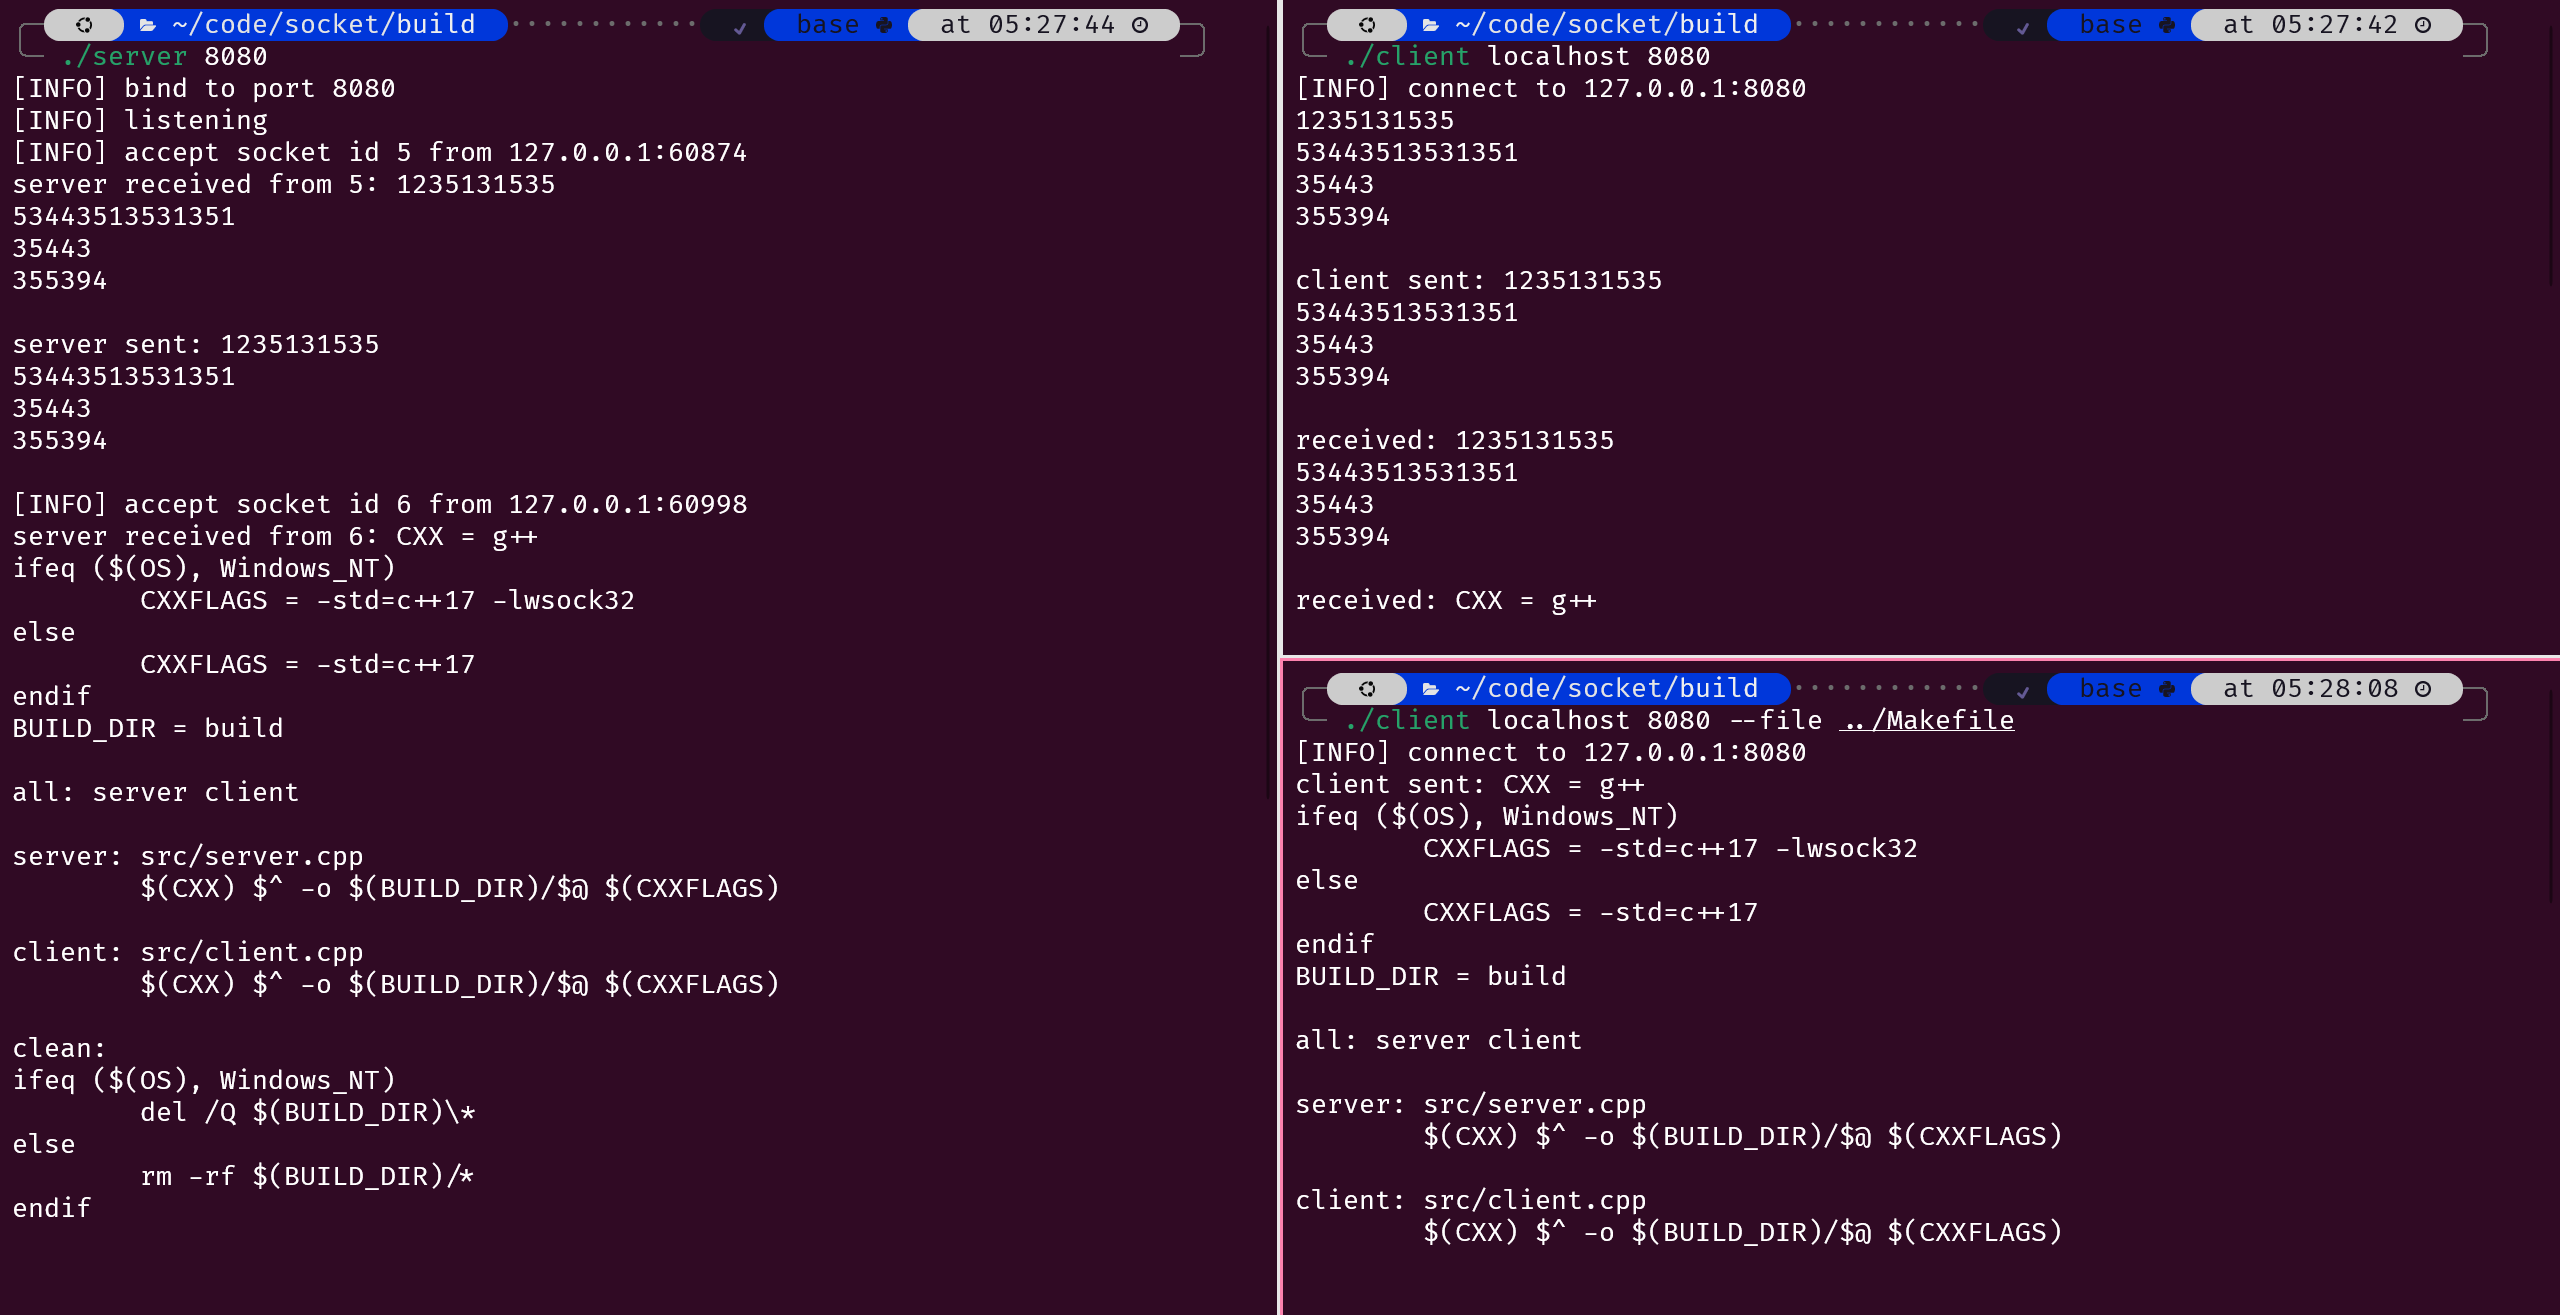
\includegraphics[width=0.95\textwidth]{img/4.png}
    \caption{能从标准输入或文件接收信息}
\end{figure}

\subsubsection{标准输入信息以两次回车作为结束标志}

在发送前进行判断即可。

\begin{lstlisting}[language=C++]
    void send(std::string_view msg) {
        if (msg.empty()) {
            if (m_last_send_enter) {
                socket::send(m_server_descriptor,
                             m_last_send + std::string{msg});
                std::cout << "client sent: " << m_last_send + std::string{msg} << std::endl;
                if (msg == "exit") {
                    close();
                }
                m_last_send_enter = false;
                m_last_send = "";
                return;
            }
            m_last_send_enter = true;
            m_last_send = "\n";
            return;
        }
        m_last_send.append(msg).append("\n");
        m_last_send_enter = true;
    }
\end{lstlisting}

\begin{figure}[H]
    \centering
    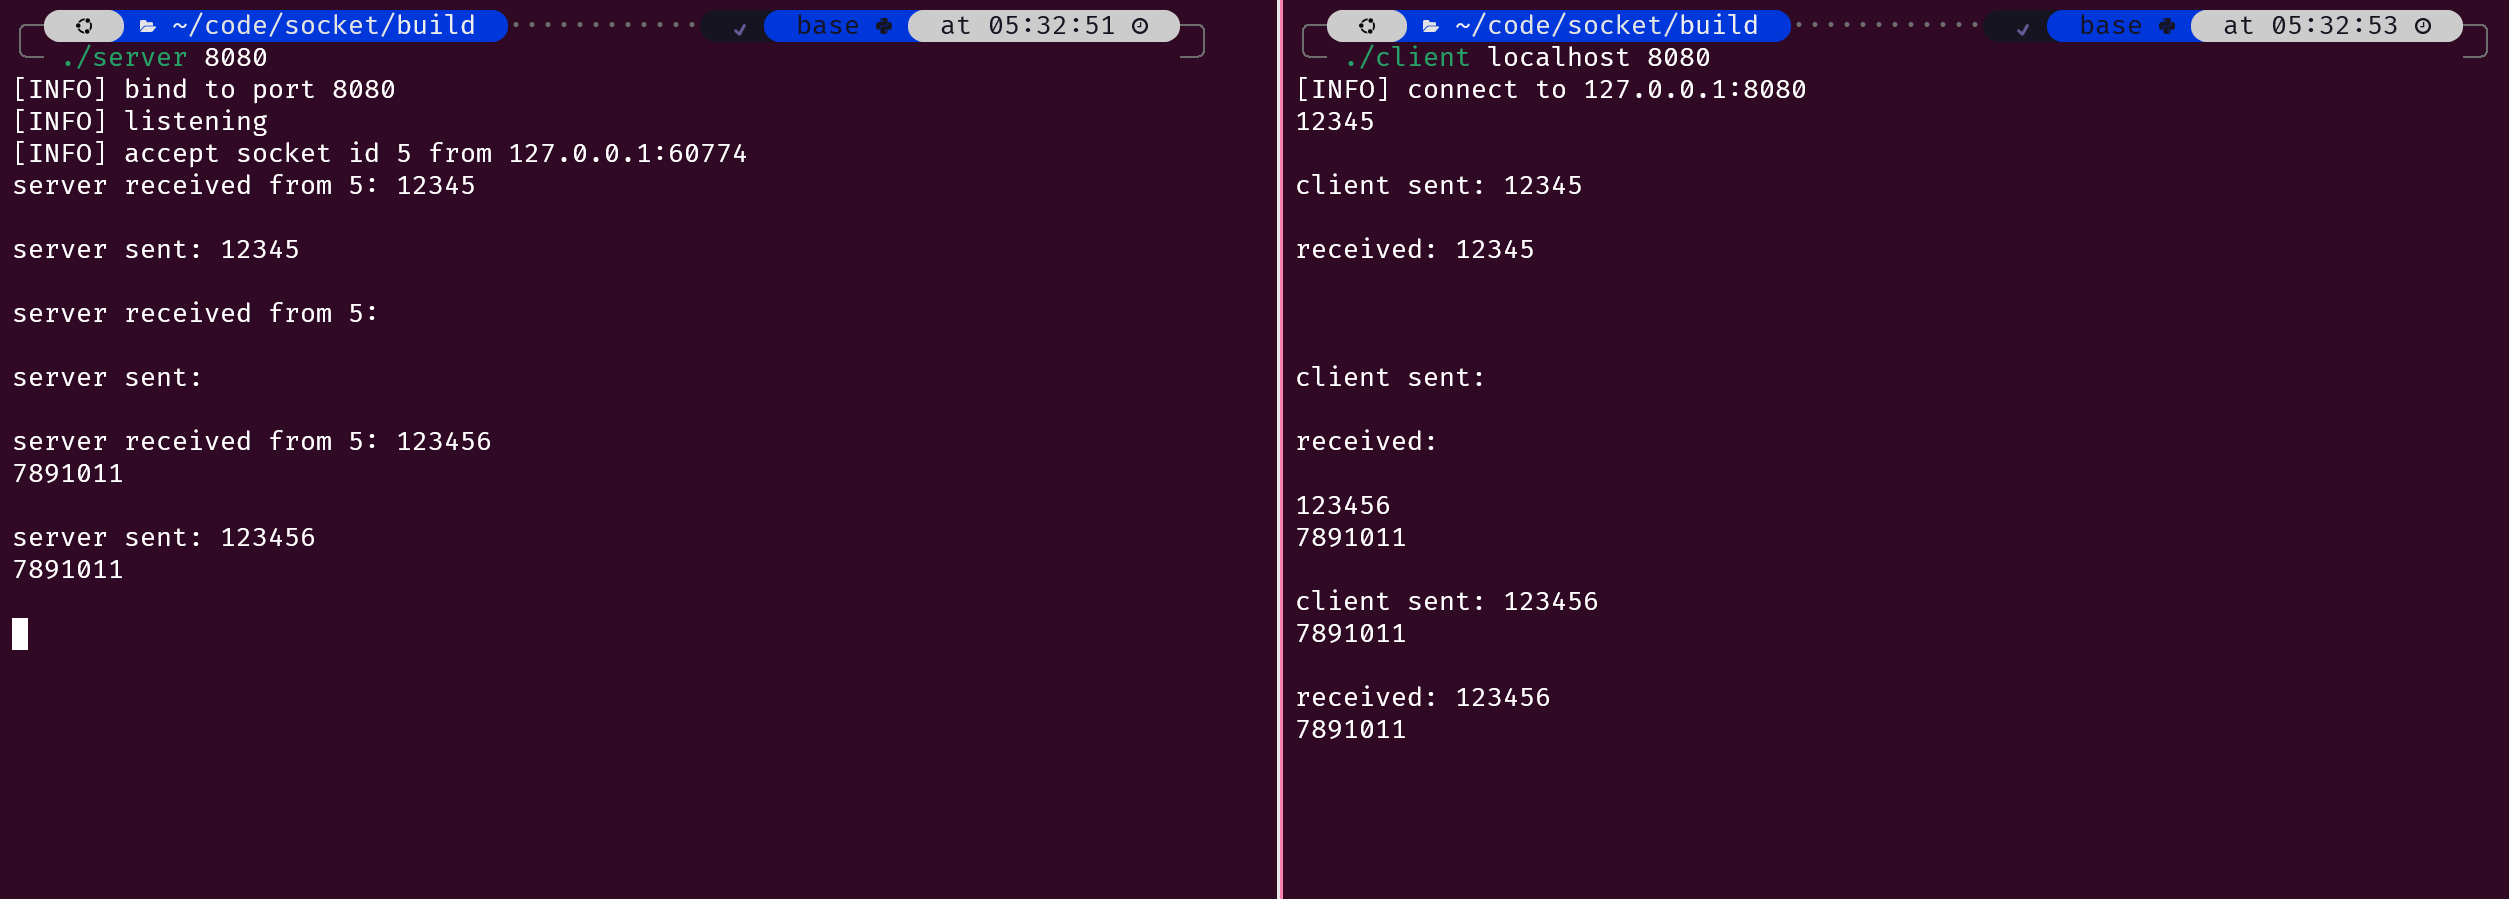
\includegraphics[width=0.95\textwidth]{img/5.png}
    \caption{标准输入信息以两次回车作为结束标志}
\end{figure}

\subsubsection{连接至错误的 \texttt{IP} 地址/端口号时能提示错误信息}

对 \texttt{IP} 地址和端口进行检查即可。

\begin{lstlisting}[language=C++]
    bool check_ipv4(std::string &addr) {
        if (addr.empty() || addr.back() == '.' || addr.front() == '.') {
            return false;
        }
        if (addr == "localhost") {
            addr = "127.0.0.1";
        }
        int num{0};
        int dot{0};
        for (auto &c : addr) {
            if (c == '.') {
                if (num < 0 || num > 255) {
                    return false;
                }
                num = 0;
                ++dot;
                continue;
            }
            if (c < '0' || c > '9') {
                return false;
            }
            num = num * 10 + (c - '0');
        }
        if (num < 0 || num > 255 || dot != 3) {
            return false;
        }
        return true;
    }
    
    // ...

    std::string ip{argv[1]};
    if (!check_ipv4(ip)) {
        std::cerr << "Invalid ip" << std::endl;
        show_usage();
        return 1;
    }

    int port{-1};
    try {
        port = std::stoi(argv[2]);
    } catch (std::exception &e) {
        std::cerr << "Invalid port" << std::endl;
        show_usage();
        return 1;
    }

    if (port < 0 || port > 65535) {
        std::cerr << "Invalid port" << std::endl;
        show_usage();
        return 1;
    }
\end{lstlisting}

\begin{figure}[H]
    \centering
    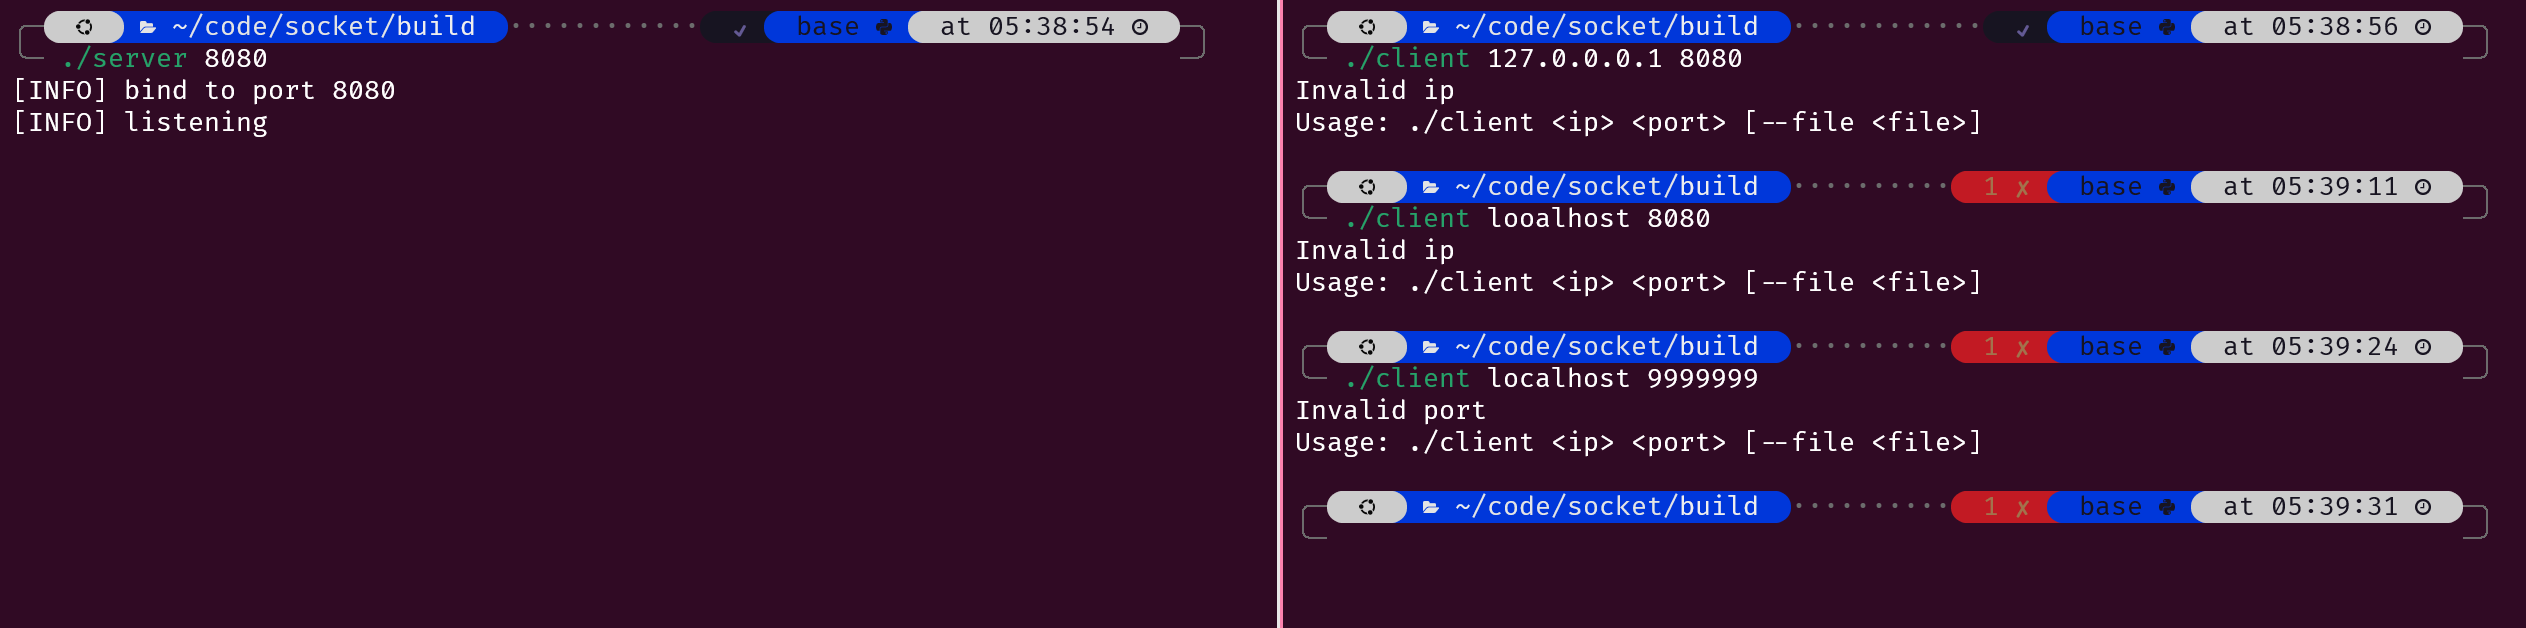
\includegraphics[width=0.95\textwidth]{img/6.png}
    \caption{连接至错误的 \texttt{IP} 地址/端口号时能提示错误信息}
\end{figure}

\subsection{整个系统}

\subsubsection{支持在 \texttt{localhost} 及两台不同机器上运行}

在 \texttt{Windows} 下, \texttt{WSL Linux}虚拟机下和手机上运行:

\begin{figure}[H]
    \centering
    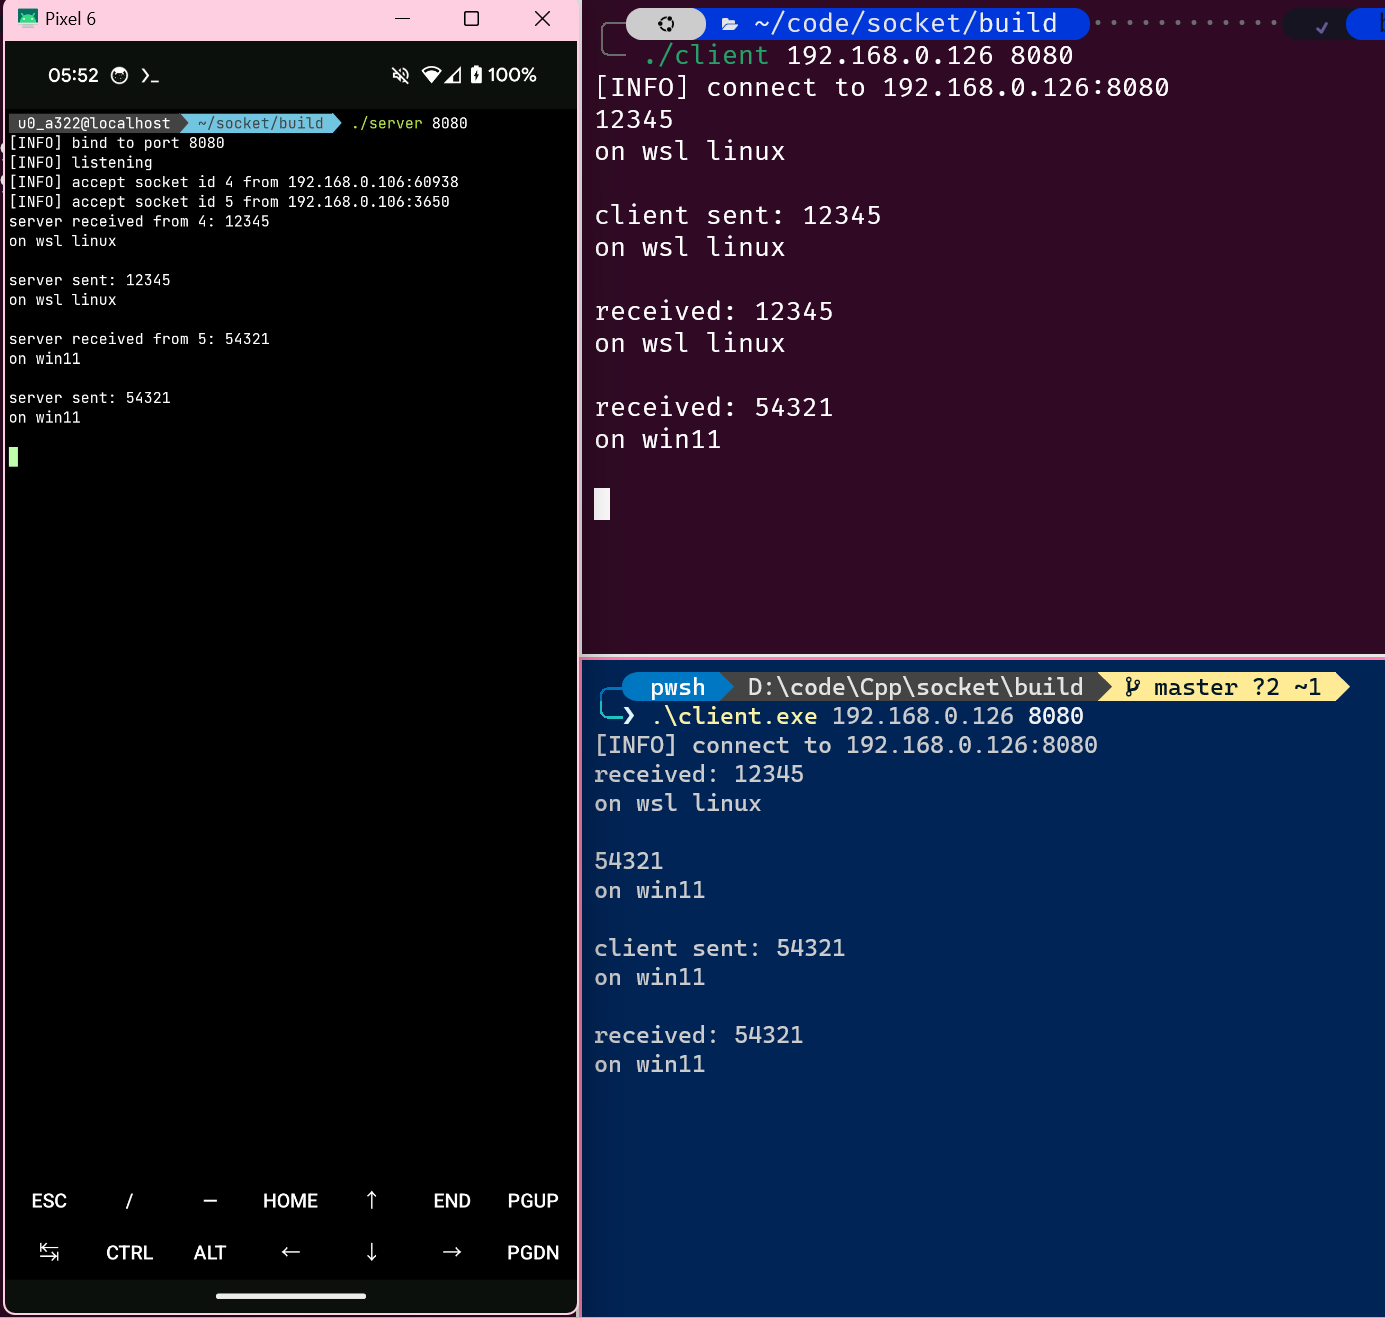
\includegraphics[width=0.95\textwidth]{img/7.png}
    \caption{支持在 \texttt{localhost} 及两台不同机器上运行}
\end{figure}

\subsubsection{支持长文本消息(不少于 \texttt{20KB})}

如下,发送 \texttt{579KB} 的文件,可以正常工作。

\begin{figure}[H]
    \centering
    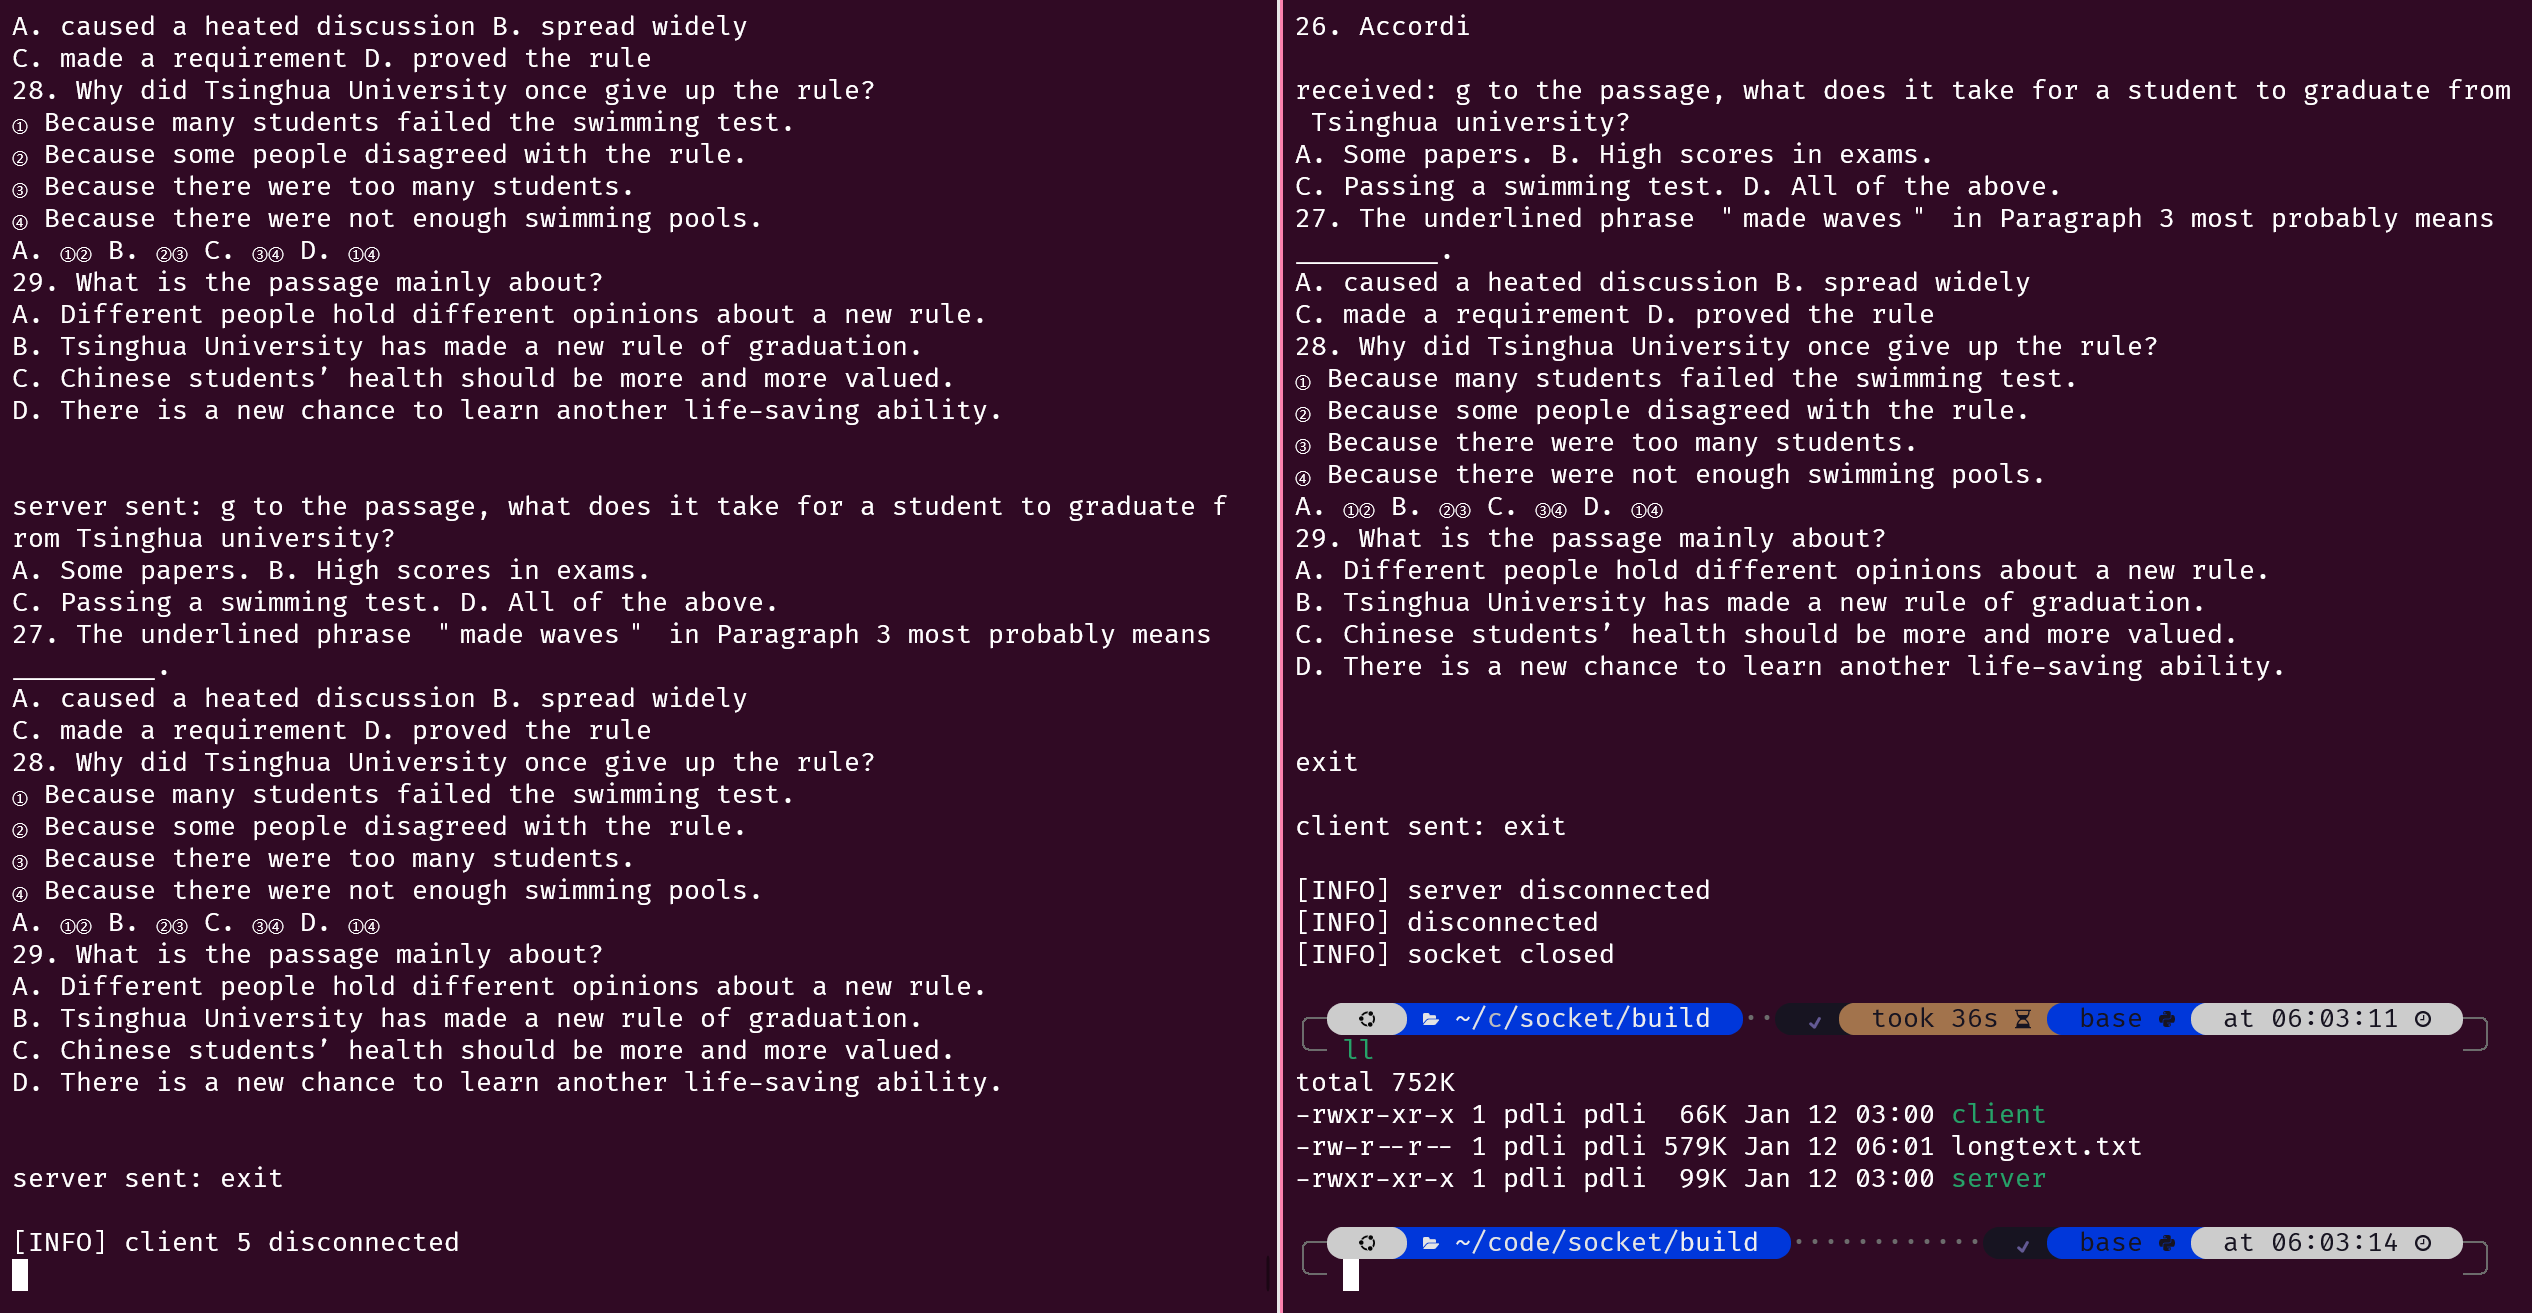
\includegraphics[width=0.95\textwidth]{img/8.png}
    \caption{支持长文本消息(不少于 \texttt{20KB})}
\end{figure}

\subsection{容错性好,无闪退}

可以正常工作,无闪退,容错性好。

\subsection{\texttt{Bonus}}

\subsubsection{支持双工通信}

在 \texttt{server} 段开启一个线程发送消息即可。

\begin{lstlisting}[language=C++]
    void input(socket_server &socket) {
        while (true) {
            std::string msg{};
            std::getline(std::cin, msg);
            socket.send_all(msg);
            if (msg == "exit") {
                socket.send_all("");
                socket.close();
                exit(0);
            }
        }
    }    
\end{lstlisting}

\begin{figure}[H]
    \centering
    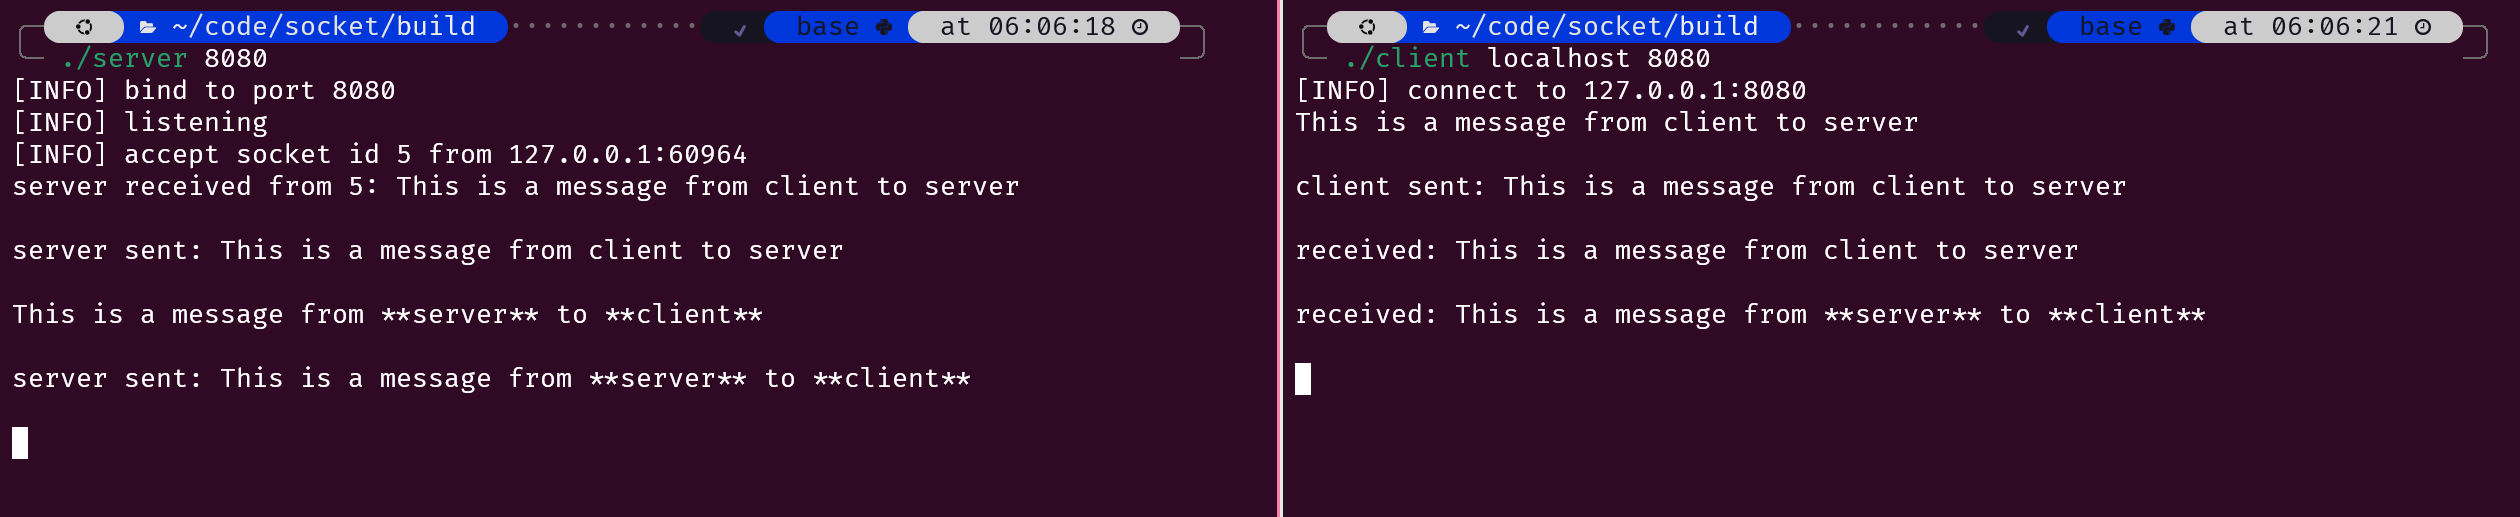
\includegraphics[width=0.8\textwidth]{img/9.png}
    \caption{支持双工通信}
\end{figure}

\section{实验结果总结}

在本次实验中,我掌握了 \texttt{socket} 编程的基本要领。

\section{附录}

\subsection{代码结构}

\begin{lstlisting}[numbers=none]
    socket
    |-- Makefile
    |-- build
    |   |-- client
    |   |-- longtext.txt
    |   `-- server
    `-- src
        |-- client.cpp
        |-- include
        |   |-- socket.hpp
        |   |-- socket_client.hpp
        |   `-- socket_server.hpp
        `-- server.cpp
    
    3 directories, 9 files
\end{lstlisting}

\subsection{源代码}

\subsubsection{\texttt{Makefile}}

\begin{lstlisting}[language=C++]
    CXX = g++
    ifeq ($(OS), Windows_NT)
        CXXFLAGS = -std=c++17 -lwsock32
    else
        CXXFLAGS = -std=c++17
    endif
    BUILD_DIR = build
    
    all: server client
    
    server: src/server.cpp
        $(CXX) $^ -o $(BUILD_DIR)/$@ $(CXXFLAGS)
    
    client: src/client.cpp
        $(CXX) $^ -o $(BUILD_DIR)/$@ $(CXXFLAGS)
    
    clean:
    ifeq ($(OS), Windows_NT)
        del /Q $(BUILD_DIR)\*
    else
        rm -rf $(BUILD_DIR)/*
    endif
\end{lstlisting}

\subsubsection{\texttt{socket.hpp}}

\begin{lstlisting}[language=C++]
    #pragma once

    #ifndef _SIMPLE_SOCKET_H_
    #define _SIMPLE_SOCKET_H_
    
    #include <iostream>
    #include <stdexcept>
    #include <string>
    #include <string_view>
    #include <unistd.h>
    
    #ifdef _WIN32
    #include <winsock2.h>
    #include <ws2tcpip.h>
    #else
    #include <arpa/inet.h>
    #include <sys/socket.h>
    #endif
    
    class socket {
      public:
        socket() : m_descriptor(-1) {
    #ifdef _WIN32
            WSADATA wsa_data;
            if (WSAStartup(MAKEWORD(2, 2), &wsa_data) != 0) {
                throw std::runtime_error("WSAStartup failed");
            }
    #endif
            m_descriptor = ::socket(AF_INET, SOCK_STREAM, 0);
            if (m_descriptor < 0) {
                throw std::runtime_error("create socket failed");
            }
        }
    
        virtual ~socket() noexcept { m_close_socket(); }
    
        void bind(int port) {
            if (port < 0 || port > 65535) {
                m_close_socket();
                throw std::runtime_error("invalid port");
            }
    
            sockaddr_in server_addr;
            server_addr.sin_family = AF_INET;
            server_addr.sin_addr.s_addr = INADDR_ANY;
            server_addr.sin_port = htons(port);
    
            if (::bind(m_descriptor, (sockaddr *)&server_addr,
                       sizeof(server_addr)) == -1) {
                m_close_socket();
                throw std::runtime_error(
                    "bind to port " + std::to_string(port) +
                    " failed\n maybe the port is already in use");
            } else {
                m_info("bind to port " + std::to_string(port));
            }
        }
    
        void listen(int n = 10) {
            if (::listen(m_descriptor, n) == -1) {
                m_close_socket();
                throw std::runtime_error("listen socket failed");
            } else {
                m_info("listening");
            }
        }
    
        int accept() {
            sockaddr_in client_addr;
            socklen_t client_addr_len = sizeof(client_addr);
            int connected =
                ::accept(m_descriptor, (sockaddr *)&client_addr, &client_addr_len);
            if (connected == -1) {
                m_close_socket();
                throw std::runtime_error("accept socket failed");
            } else {
                m_info("accept socket id " + std::to_string(connected) + " from " +
                       std::string(inet_ntoa(client_addr.sin_addr)) + ":" +
                       std::to_string(ntohs(client_addr.sin_port)));
            }
            return connected;
        }
    
        int connect(const char *ip, int port) {
            sockaddr_in server_addr;
            server_addr.sin_family = AF_INET;
            server_addr.sin_addr.s_addr = inet_addr(ip);
            server_addr.sin_port = htons(port);
    
            int connected = ::socket(AF_INET, SOCK_STREAM, 0);
    
            if (::connect(connected, (sockaddr *)&server_addr,
                          sizeof(server_addr)) == -1) {
                m_close_socket();
                throw std::runtime_error("connect to " + std::string(ip) + ":" +
                                         std::to_string(port) + " failed");
            } else {
                m_info("connect to " + std::string(ip) + ":" +
                       std::to_string(port));
            }
            return connected;
        }
    
        int connect(std::string ip, int port) { return connect(ip.c_str(), port); }
    
        int connect(std::string_view ip, int port) {
            return connect(ip.data(), port);
        }
    
        void send(int to, const char *data, int len) {
            if (::send(to, data, len, 0) == -1) {
                m_error("send data to " + std::to_string(to) + " failed");
            }
        }
    
        void send(int to, std::string_view data) {
            send(to, data.data(), data.size());
        }
    
        bool recv(int from, char *data, int len) {
            int read_num = ::recv(from, data, len, 0);
            if (read_num == -1) {
                m_error("recv data from " + std::to_string(from) + " failed");
                return false;
            }
            if (read_num == 0) {
                return false;
            }
            return true;
        }
    
        void close() { m_close_socket(); }
    
      private:
        int m_descriptor;
    
        void m_close_socket() {
            if (m_descriptor != -1) {
                m_info("socket closed");
                ::close(m_descriptor);
                m_descriptor = -1;
            }
        }
    
        void m_info(const std::string &msg) {
            std::cout << "[INFO] " << msg << std::endl;
        }
    
        void m_error(const std::string &msg) {
            std::cerr << "[ERROR] " << msg << std::endl;
        }
    };
    
    #endif // _SIMPLE_SOCKET_H_    
\end{lstlisting}

\subsubsection{\texttt{socket\_client.hpp}}

\begin{lstlisting}[language=C++]
    #pragma once

    #ifndef _CLIENT_H_
    #define _CLIENT_H_
    
    #include "socket.hpp"
    #include <cstring>
    #include <iostream>
    #include <unistd.h>
    
    class socket_client : socket {
    public:
        socket_client()
            : socket(), m_server_descriptor(-1), m_last_send_enter(false) {}
    
        void connect(std::string_view ip, int port) {
            m_server_descriptor = socket::connect(ip, port);
        }
    
        void send(std::string_view msg) {
            if (msg.empty()) {
                if (m_last_send_enter) {
                    socket::send(m_server_descriptor,
                                 m_last_send + std::string{msg});
                    std::cout << "client sent: " << m_last_send + std::string{msg} << std::endl;
                    if (msg == "exit") {
                        close();
                    }
                    m_last_send_enter = false;
                    m_last_send = "";
                    return;
                }
                m_last_send_enter = true;
                m_last_send = "\n";
                return;
            }
            m_last_send.append(msg).append("\n");
            m_last_send_enter = true;
        }
    
        std::string recv(int size = 1024) {
            char* buffer = new char[size];
            std::memset(buffer, 0, size);
            bool ok = socket::recv(m_server_descriptor, buffer, size);
            auto res = std::string(buffer);
            delete[] buffer;
            if (!ok || res == "exit\n") {
                res = "";
                std::cout << "[INFO] server disconnected" << std::endl;
                close();
            }
            return res;
        }
    
        void close() {
            if (m_server_descriptor != -1) {
                std::cout << "[INFO] disconnected" << std::endl;
                ::close(m_server_descriptor);
                m_server_descriptor = -1;
            }
            socket::close();
        }
    
    private:
        int m_server_descriptor;
        bool m_last_send_enter;
        std::string m_last_send{};
    };
    
    #endif // _CLIENT_H_    
\end{lstlisting}

\subsubsection{\texttt{socket\_server.hpp}}

\begin{lstlisting}[language=C++]
    #pragma once

    #ifndef _SERVER_H_
    #define _SERVER_H_
    
    #include "socket.hpp"
    #include <cstring>
    #include <iostream>
    #include <vector>
    
    class socket_server : socket {
      public:
        socket_server() : socket() {}
    
        void bind(int port) { socket::bind(port); }
    
        void listen(int n = 10) { socket::listen(n); }
    
        int accept() {
            int connected = socket::accept();
            m_connections.push_back(connected);
            return connected;
        }
    
        void send_all(std::string_view msg) {
            if (msg.empty()) {
                if (m_last_send_enter) {
                    m_send_all(m_last_send + std::string{msg});
                    std::cout << "server sent: " << m_last_send + std::string{msg}
                              << std::endl;
                    if (msg == "exit") {
                        close();
                    }
                    m_last_send_enter = false;
                    m_last_send = "";
                    return;
                }
                m_last_send_enter = true;
                m_last_send = "\n";
                return;
            }
            m_last_send.append(msg).append("\n");
            m_last_send_enter = true;
        }
    
        void send(int to, std::string_view msg) {
            if (msg.empty()) {
                if (m_last_send_enter) {
                    socket::send(to, m_last_send + std::string{msg});
                    if (msg == "exit") {
                        m_close(to);
                        return;
                    }
                    std::cout << "server sent: " << m_last_send + std::string{msg}
                              << std::endl;
                    m_last_send_enter = false;
                    m_last_send = "";
                    return;
                }
                m_last_send_enter = true;
                m_last_send = "\n";
                return;
            }
            m_last_send.append(msg).append("\n");
            m_last_send_enter = true;
        }
    
        const std::string recv(int from, int size = 1024) {
            char *buffer = new char[size];
            std::memset(buffer, 0, size);
            bool ok = socket::recv(from, buffer, size);
            auto res = std::string(buffer);
            delete[] buffer;
            if (!ok || res == "exit\n") {
                send(from, "exit");
                send(from, "");
                std::cout << "[INFO] client " << from << " disconnected"
                          << std::endl;
                m_close(from);
                res = "";
            }
            return res;
        }
    
        void close() { socket::close(); }
    
      private:
        std::vector<int> m_connections{};
    
        bool m_last_send_enter{false};
    
        std::string m_last_send{};
    
        void m_close(int client) {
            for (auto it = m_connections.begin(); it != m_connections.end(); ++it) {
                if (*it == client) {
                    m_connections.erase(it);
                    break;
                }
            }
        }
    
        void m_send_all(std::string_view msg) {
            for (auto &client : m_connections) {
                socket::send(client, msg);
            }
        }
    };
    
    #endif // _SERVER_H_    
\end{lstlisting}

\subsection{\texttt{client.cpp}}

\begin{lstlisting}[language=C++]
    #include "include/socket_client.hpp"
    #include <exception>
    #include <fstream>
    #include <iostream>
    #include <string>
    #include <thread>
    
    bool check_ipv4(std::string &addr) {
        if (addr.empty() || addr.back() == '.' || addr.front() == '.') {
            return false;
        }
        if (addr == "localhost") {
            addr = "127.0.0.1";
        }
        int num{0};
        int dot{0};
        for (auto &c : addr) {
            if (c == '.') {
                if (num < 0 || num > 255) {
                    return false;
                }
                num = 0;
                ++dot;
                continue;
            }
            if (c < '0' || c > '9') {
                return false;
            }
            num = num * 10 + (c - '0');
        }
        if (num < 0 || num > 255 || dot != 3) {
            return false;
        }
        return true;
    }
    
    void receive(socket_client &socket) {
        while (true) {
            auto msg = socket.recv();
            if (msg.empty()) {
                socket.close();
                exit(0);
            }
            std::cout << "received: " << msg << std::endl;
        }
    }
    
    int main(const int argc, const char **argv) {
        const auto show_usage = [argv]() {
            std::cerr << "Usage: " << argv[0] << " <ip> <port> [--file <file>]"
                      << std::endl;
        };
    
        if ((argc != 3 && argc != 5) ||
            (argc == 5 && std::string{argv[3]} != "--file")) {
            std::cerr << "Invalid arguments" << std::endl;
            show_usage();
            return 1;
        }
    
        std::string ip{argv[1]};
        if (!check_ipv4(ip)) {
            std::cerr << "Invalid ip" << std::endl;
            show_usage();
            return 1;
        }
    
        int port{-1};
        try {
            port = std::stoi(argv[2]);
        } catch (std::exception &e) {
            std::cerr << "Invalid port" << std::endl;
            show_usage();
            return 1;
        }
    
        if (port < 0 || port > 65535) {
            std::cerr << "Invalid port" << std::endl;
            show_usage();
            return 1;
        }
    
        socket_client client{};
        client.connect(ip, port);
    
        std::thread recv_t(receive, std::ref(client));
    
        if (argc == 5) {
            std::fstream in{argv[4]};
            std::string str{};
            std::string tmp{};
            while (std::getline(in, tmp)) {
                str.append(tmp).append("\n");
            }
            client.send(str);
            client.send("");
        }
    
        while (true) {
            std::string msg;
            std::getline(std::cin, msg);
            client.send(msg);
        }
    
        recv_t.join();
    }    
\end{lstlisting}

\subsubsection{\texttt{server.cpp}}

\begin{lstlisting}[language=C++]
    #include "include/socket_server.hpp"
    #include <functional>
    #include <iostream>
    #include <thread>
    
    void handle_connection(socket_server &socket, int client) {
        while (true) {
            auto msg = socket.recv(client);
            if (msg.empty()) {
                break;
            }
            std::cout << "server received from " << client << ": " << msg
                      << std::endl;
            msg = msg.substr(0, msg.size() - 1);
            socket.send_all(msg == "\n" ? "" : msg);
            socket.send_all("");
        }
    }
    
    void input(socket_server &socket) {
        while (true) {
            std::string msg{};
            std::getline(std::cin, msg);
            socket.send_all(msg);
            if (msg == "exit") {
                socket.send_all("");
                socket.close();
                exit(0);
            }
        }
    }
    
    int main(const int argc, const char **argv) {
        const auto show_usage = [argv]() {
            std::cerr << "Usage: " << argv[0] << " <port>" << std::endl;
        };
    
        if (argc != 2) {
            show_usage();
            return 1;
        }
    
        int port{-1};
        try {
            port = std::stoi(argv[1]);
        } catch (std::exception &e) {
            std::cerr << "Invalid port" << std::endl;
            show_usage();
            return 1;
        }
    
        if (port < 0 || port > 65535) {
            std::cerr << "Invalid port" << std::endl;
            show_usage();
            return 1;
        }
    
        socket_server server{};
    
        server.bind(port);
        server.listen();
    
        std::vector<std::thread> threads{};
    
        std::thread input_t{input, std::ref(server)};
    
        while (true) {
            int client = server.accept();
            threads.emplace_back(handle_connection, std::ref(server), client);
        }
    
        for (auto &thread : threads) {
            thread.join();
        }
    }    
\end{lstlisting}
\end{document}